\chapter{Metod}
\label{cha:method}
Det här kapitlet beskriver hur projektet har utförts samt beskrivningar av de metoder och verktyg som använts för de olika områden projektet omfattar.

\section{Projektorganisation}
Teamet består av 8 teammedlemmar. Den utförda kursen omfattade några förbestämda roller som skulle tilldelas till teammedlemmarna. Rollerna delades upp efter en intern valprocess vid projektets start. Rollerna är väldefinierade och dess ansvarsområden beskrivs nedan.

\subsubsection*{Teamledare -- Alexander Wilkens}
Teamledaren ska se till att samtliga processer som ska utföras under projektets gång följs. Denna person representerar också teamet utåt och har kontakt med handledaren. Om det behövs har teamledaren sista ordet.

\subsubsection*{Kvalitetssamordnare -- Joel Almqvist}
Kvalitetssamordnaren ansvarar för arbetsprocesser som ska hålla kvaliteten av projektet på en hög nivå. Samordnaren gör en budget av vad kvalitet får kosta, samtidigt som han ansvarar för kvalitetsplanen.

\subsubsection*{Dokumentansvarig -- Tim Håkansson}
Dokumentansvarig ansvarar för samtliga dokument som teamet ska producera. Rollen är även ansvarig för gruppens logotyp och dokumentmallar.

\subsubsection*{Arkitekt -- Joel Oskarsson}
Rollen arkitekt ansvarar för arkitekturen av den tekniska delen av projektet. Arkitekten ansvarar även för övergripande teknikval och har det sista ordet på tekniska beslut.

\subsubsection*{Utvecklingsledare -- Lieth Wahid}
Utvecklingsledaren ansvarar för den mer detaljerade designen av den tekniska produkten, leder utvecklingsarbetet och ser till att resten av teamet har något att arbeta med.

\subsubsection*{Analysansvarig -- Axel Löjdquist}
Analysansvarig ansvarar för majoriteten av kundkontakt och jobbar ständigt med att ta reda på kundens verkliga behov. Huvudansvaret för kravspecifikationen ligger på denna roll.

\subsubsection*{Testledare -- David Kjellström}
Testledaren beslutar systemets status genom att arbeta tillsammans med kvalitetssamordnaren för att testa så systemet uppnår kraven. Testledaren skriver testplan och testrapport.

\subsubsection*{Konfigurationsansvarig -- Björn Detterfelt}
Konfigurationsansvarig ansvarar för generell versionshantering i projektet. Rollen arbetar mycket med utvecklingsledaren och dokumentansvarig för att bestämma vilka arbetsprodukter som ska ingå i en utgåva.

\section{Utvecklingsmetodik}
Det här avsnittet beskriver utvecklingsmetodiken projektgruppen har följt. Detta innefattar hur olika metoder och verktyg har använts för att uppnå ett resultat.

\subsection{Projektfaser}
Nedan beskrivs faserna projektet uppdelades i.

\subsubsection*{Förstudier}
Första fasen under projektet bestod av att göra förstudier inför projektet. Detta inkluderar skrivandet av diverse dokument som beskrivs under avsnitt \ref{sec:method-documentation}. Dessutom gjordes individuella studier om Javascript och olika bibliotek så alla lättare skulle kunna börja arbeta under utvecklingen. I slutet av förstudierna gavs även en workshop av Cybercom om deras backend.

\subsubsection*{Utveckling}
Själva utvecklingen utfördes mestadels på Cybercoms kontor för att teamet lättare skulle kunna ställa frågor om funderingar som uppkom. En annan fördel var att teamet hade tillgång till en gemensam arbetsplats.

\subsubsection*{Kvalitetssäkring}
Under denna fas finslipades diverse funktioner för att ge användaren en bättre upplevelse när de använder produkten. Detta inkluderade buggfixar och verifiering av projektets kravspecifikation.

\subsubsection*{Efterstudier}
Efter projektet gjordes efterstudier för att granska det resultat teamet fick för att göra en utvärdering av projektet.

\subsection{Utvecklingsmetod} \label{main:Scrum}
Projektgruppen bestämde tidigt att utveckla med det agila ramverket Scrum med modifikationer. Delarna från ramverket som valdes till projektet var \textit{sprintutvärdering}, \textit{sprint-backlog}, \textit{produkt-backlog}, \textit{Scrum-bräde} och \textit{sprintplanering}. Resterande delar från ramverket valdes bort då projektgruppen tyckte koncepten kändes onödiga för projektet. Vid början av varje sprint samlades projektgruppen för att organisera en \textit{sprint-backlog} från \textit{produkt-backlogen}. \textit{Produkt-backlogen} uppdaterades med aktiviteter kontinuerligt av alla medlemmar när en aktivitet upptäcktes. Projektet bestod av tre olika kodbaser. Varje aktivitet hade en eller flera tillhörande etiketter som beskrev vilka kodbaser aktiviteten berörde. Detta gjorde att ett gemensamt \textit{Scrum-bräde} kunde användas för samtliga kodbaser. Vid slutet av varje sprint utvärderades sprinten i form av ett kortare möte där varje projektmedlem kunde uttrycka sina åsikter kring utvecklingsprocessen.

Verktyget Trello användes för att organisera och representera ett \textit{Scrum-bräde} under projektets gång. På detta bräde fanns kolumnerna ``aktiviteter'', ``att göra'', ``implementeras'', ``väntar'' och ``klar''. I kolumnen ``aktiviteter'' hamnade alla aktiviteter som behövde utföras för att få en färdig produkt. Aktiviteter kunde läggas till i denna kolumn under en pågående sprint. Kolumnen ``att göra'' fylldes på med aktiviteter som förväntades bli klara under en pågående sprint. Varje aktivitet tilldelades en prioritet, en tidsestimering och en beskrivning. Dessa attribut sattes under \textit{sprintplaneringen} och hjälpte gruppen att belasta varje sprint med en rimlig mängd aktiviteter. I ``implementeras'' hamnade alla aktiviteter som en eller flera projektmedlemmar arbetade med. I ``väntar'' hamnade alla aktiviteter som påbörjats men stoppats på grund av andra prioriteringar. I ``klar'' hamnade alla aktiviteter som blivit avklarade. Denna kolumn användes som en logg över vad som hade gjorts under en sprint och som underlag för \textit{sprintutvärderingar}. En bild på en av gruppens Scrum-bräden kan ses i figur \ref{fig:trello_board}.

\begin{figure}[h]
    \centering
    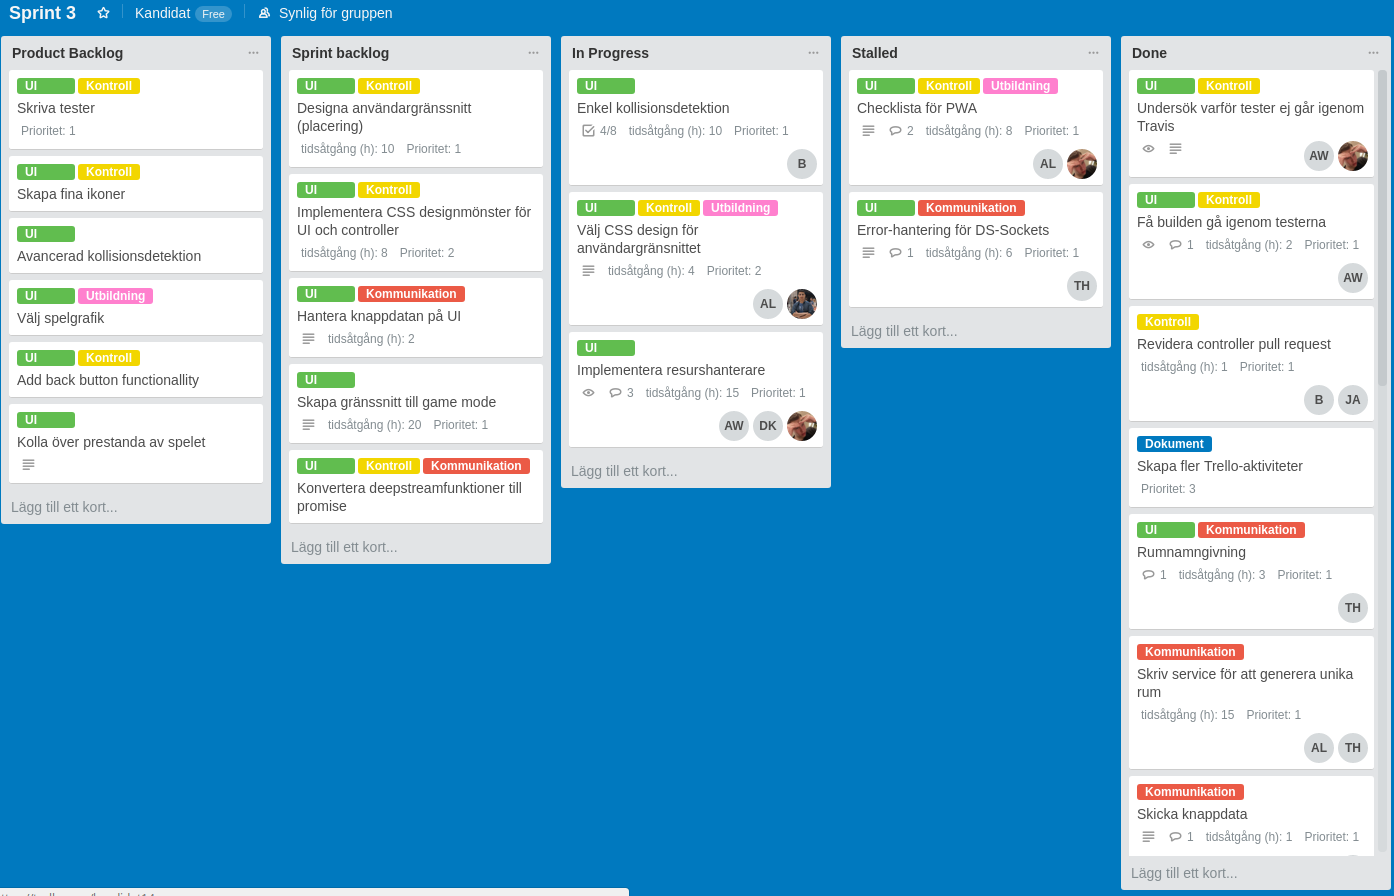
\includegraphics[scale=0.43]{trello_board}
    \caption{En skärmbild av gruppens \textit{Scrum-bräde} för sprint 3}
    \label{fig:trello_board}
\end{figure}

\subsection{Versionshantering}
Git användes för att versionshantera koden. Själva Git-repot lagrades på Github för att alla lätt skulle kunna ladda ner och ladda upp filer till ett centralt repo. Dessutom kan GitHub hantera diverse tester så att endast kod som går igenom våra tester kan laddas upp på master-grenen.

Utöver det så fungerar master-grenen som en form av intern utgåva av produkten. Det vill säga att produkten ska vara körbar och fungera som väntat i denna gren. För att garantera detta laddades aldrig kod upp direkt till grenen utan det krävdes en pull request som godkändes av en annan projektmedlem. För att en pull request ska bli godkänd ska granskaren läsa igenom koden och testa relevanta områden för att garantera att det fungerar som det ska.

\subsection{Testning}
Under förstudiefasen undersökte testledaren vilka verktyg som kunde användas för projektet samt hur hela testningsprocessen skulle gå till. Projektgruppen beslutade om att verktyget Travis skulle användas för automatiska tester, men även manuella tester skulle utföras. De automatiska testerna användes främst för enhetstest medan de manuella testerna användes för mer komplicerade integrationstest.

De manuella testerna baserades på krav specificerade i kravspecifikationen. Efter att ett manuellt test hade utförts skrevs en testrapport för det utförda testet. Testrapporten innehåller varje utfört steg i testet, dess förväntade resultat och det faktiska resultatet. Dessa tester utfördes främst vid projektets slut för att verifiera att de specificerade kraven uppfylldes.

Travis är ett verktyg som kör förskrivna tester vid varje pull request eller push till en gren. Om dessa tester skulle misslyckas vid en pull request från master-grenen nekas integrationen. En push kommer alltid lyckas även vid ett misslyckat test, men Travis noterar att testet har misslyckats.

Huvudsyftet för de automatiska testerna var att se till att ingen felaktigkod fanns på master-grenen. Testerna kontrollerar att koden kompilerar, att det inte finns några Eslint-fel samt att de egenskrivna testerna uppfylls. Automatiska tester skrevs under utvecklingens gång. När ny funktionalitet implementerades skrevs även tester till denna.

\subsection{Möten}
Vid början av varje vecka hade projektgruppen ett möte för att diskutera vad som skulle hända framöver och där funderingar eller problem kunde tas upp och diskuteras. Dessutom hade projektgruppen ett handledarmöte varje vecka. På handledarmötet kunde generella frågor kring projektet ställas och vägledning gavs för diverse problem eller funderingar projektgruppen hade. Alla möten dokumenterades med hjälp av ett mötesprotokoll som projektgruppen formulerat.

En gemensam Google-kalender skapades där alla möten samt viktiga moment och deadlines lades till. Alla moment som lades till i kalendern ansågs vara obligatoriska av projektgruppen där alla medlemmar förväntades medverka.

\subsection{Kommunikation}
Kommunikationen mellan externa parter och projektgruppen gick i huvudsak genom rollerna teamledare och analysansvarig. Slack användes för både den interna och externa kommunikationen under projektets gång. En Slack-arbetsplats skapades, där enbart projektgruppen var medlemmar. Majoriteten av den interna kommunikationen skedde genom denna. Olika kanaler skapades på denna Slack-arbetsplats för att diskutera olika ärenden och hålla kommunikationen strukturerad. Det fanns ytterligare en Slack-arbetsplats där både projektgruppen och kunden medverkade. På denna arbetsplats skedde en del av den externa kommunikationen med kunden. Kommunikation skedde även muntligt med kunden ute på deras kontor. Även denna arbetsplats var uppdelad i olika kanaler: frågor och allmänt. Tanken bakom kanalen frågor var att projektgruppen kunde fylla kanalen med frågor rörande utvecklingen och kunden kunde bearbeta frågorna när de hade tid. Kanalen allmänt användes för all övrig kommunikation.

\subsection{Enkät och demonstationer}
\label{sec:method-poll}
För att verifiera att produkten håller hög kvalitet bestämde gruppen sig för att genomföra en enkätundersökning. I denna undersökning fick 20 personer testa att använda produkten och sedan fylla i en enkät gällande upplevelsen. De valda testpersonerna kom från två grupper, studenter slumpmässigt valda på Linköpings universitets campus och anställda på Cybercom. Dessa personer fick testa spelet i ungefär fem minuter innan de fick fylla i enkäten med nedanstående frågor. På varje fråga fick ett betyg ges mellan ett och tio där ett är helt emot och tio betyder att man instämmer helt.


\begin{enumerate}[label={(\alph*)}]
	\item Jag tycker det var svårt att förstå spelets regler.
	\item Jag tycker att spelet kändes responsivt. (Spelpjäsen rörde sig på ett bra sätt efter mina rörelser)
	\item Jag tycker det var lätt att följa vad som hände på den stora spelskärmen.
	\item Jag tycker spelet var kul.
	\item Jag tycker det var lätt att styra min spelpjäs.
\end{enumerate}

Utöver testtillfällena med enkäten har också demonstationer för kunden förekommit. Dessa demonstationer har både varit informella, i form av snabbt visa upp vad som gjorts under exempelvis dagen, och formella. De formella demonstationerna var presentationer till kund kring hur produkten såg ut. Kunden fick chans att både spela spelet men också ställa frågor kring implementation och design som ansågs vara intressant.


\section{Dokumentation}
\label{sec:method-documentation}
Det här avsnittet beskriver vilka verktyg som har använts för att dokumentera projektgruppens arbete samt vilka dokument som har producerats och dess syften.

\subsection{Dokument}
Nedan beskrivs alla dokument projektgruppen producerat.

\subsubsection*{Projektplan}
Projektplan består av en beskrivning utav projektet, resurser som teamet har tillgång till, processer som kommer användas och risker inom projektet. Dessutom beskrivs en aktivitetsplan som översiktligt tar upp alla aktiviteter som kommer att
göras under projektet.

\subsubsection*{Kravspecifikation}
Kravspecifikationen förtydligar vad som förväntas vara klart vid projektets slut. Dokumentet fungerar som överenskommelse mellan kunden och projektgruppen. Kraven specificerar vilken funktionalitet, kvalitet och design, produkten ska uppfylla. Dokumentet utgör grunden för hur hela projektet ska struktureras och utformas. Kraven är framtagna efter kundens önskemål och formulerade för att ligga till stöd för projektgruppens arbete.

\subsubsection*{Kvalitetsplan}
Kvalitetsplanen definierar processer vars syften är att säkerställa att produkten håller en hög kvalitet. Kvaliteterna som är i huvudfokus är definierade i kravspecifikationen och är baserade på kundens önskemål.

\subsubsection*{Statusrapport}
Statusrapporten är som en mindre projektplan för
de olika iterationerna. Rapporten reflekterar över hur allt förarbete har gått, vad som kommer
hända till nästa iteration samt vilka risker projektgruppen står inför.

\subsubsection*{Systemanatomi}
Anatomin för systemet beskriver hur systemet är uppbyggt på olika nivåer, såsom funktioner, mjukvara, hårdvara. Anatomin ger en större bild för hur systemet fungerar och beskriver vilken miljö den kommer befinna sig i.

\subsubsection*{Arkitekturbeskrivning}
Arkitekturbeskrivningen detaljerar arkitekturen för systemet samt beskriver hur olika submoduler hänger ihop. Arkitekturens fördelar, nackdelar och möjliga utökningar förklaras även i dokumentet.

\subsubsection*{Testplan}
Testplanen beskriver hur de olika delarna av produkten ska testas och även hur man ska följa upp på testerna.

\subsubsection*{Gruppkontrakt}
Projektgruppen producerade och undertecknade ett gruppkontrakt som skrevs vid ett tidigt stadie för att förtydliga vad som förväntades av varje gruppmedlem.

\subsubsection*{Tidrapport}
Tidrapporteringen under projektet skedde i ett Excel blad där varje teammedlem rapporterade den tid de har spenderat under en dag. Tiderna som skrevs ner fick inte överstiga två timmar och arbetspass som varade längre skrevs som två eller flera olika arbetstillfällen. Detta för att få en bättre bild av vad som har jobbats på under arbetspassen. I och med tidsrapporteringen kunde även en \textit{burndown chart}genereras för att få en bättre uppfattning om hur teamet låg till i tidsåtgång.

\subsubsection*{Mötesprotokoll}
Under projektet hölls olika möten för att diskutera saker som har kommit upp. Alla möten dokumenterades genom en mötesprotokollmall som skrevs vid varje möte.

\subsection{Dokumentskrivning}
Själva dokumentskrivningen utfördes genom att skriva i Latex, vilket gjorde det lättare att dela upp dokumenten i olika sektioner. Utöver Latex användes Google Drive för mer inofficiella dokument såsom mötesprotokoll, veckorapporter och seminarieförberedelser.

\subsection{Dokumentlagring}
Dokumenten som skapades under projektets gång lagrades på Google Drive för att både versionshantera de olika färdiga iterationerna av dokumenten, men även för att enkelt kunna se dokumenten om Latax inte finns till hand. Dessutom versionshanterades dokumenten under arbetets gång med hjälp av Git genom Github. Detta hjälpte dokumentskrivning genom att hantera olika konflikter när olika personer sitter i samma fil och skriver.

\section{Metod för att fånga erfarenheter}
Då teamet är samlat från olika program på universitetet och alla har olika erfarenheter om olika områden, vare sig det gäller spelprogrammering eller generell Javascript, behövdes det en struktur för att samla och ta nytta av varje projektmedlems kunskaper. För att uppnå detta samlade teamet in och skrev ner de olika kunskaperna som teamet hade och utifrån det höll olika workshops för att få alla projektmedlemmar på ungefär samma nivå.

Utöver det jobbade teamet i grupper om två till tre vilket underlättade arbetet då man lättare kunde utbyta erfarenheter. Dessa grupper växlades även vid jämna mellanrum så alla kunde del av alla andras erfarenheter. Hela gruppen delade även med sig av problem och nya erfarenheter på de regelbundna mötena. Dessa antecknades i mötesprotokollen.
